\documentclass{exam}

\usepackage{siunitx} 
\usepackage{graphicx}
\usepackage[fleqn]{amsmath}
\usepackage{cancel}
\usepackage{float}
\usepackage{mdwlist}
\usepackage{booktabs}
\usepackage{cancel}
\usepackage{polynom}
\usepackage{caption}
\usepackage{fullpage}
\usepackage{comment}
\usepackage{enumerate}

\newcommand{\degree}{\ensuremath{^\circ}} 
\everymath{\displaystyle}

% \begin{figure}[H]
%   \centering
%   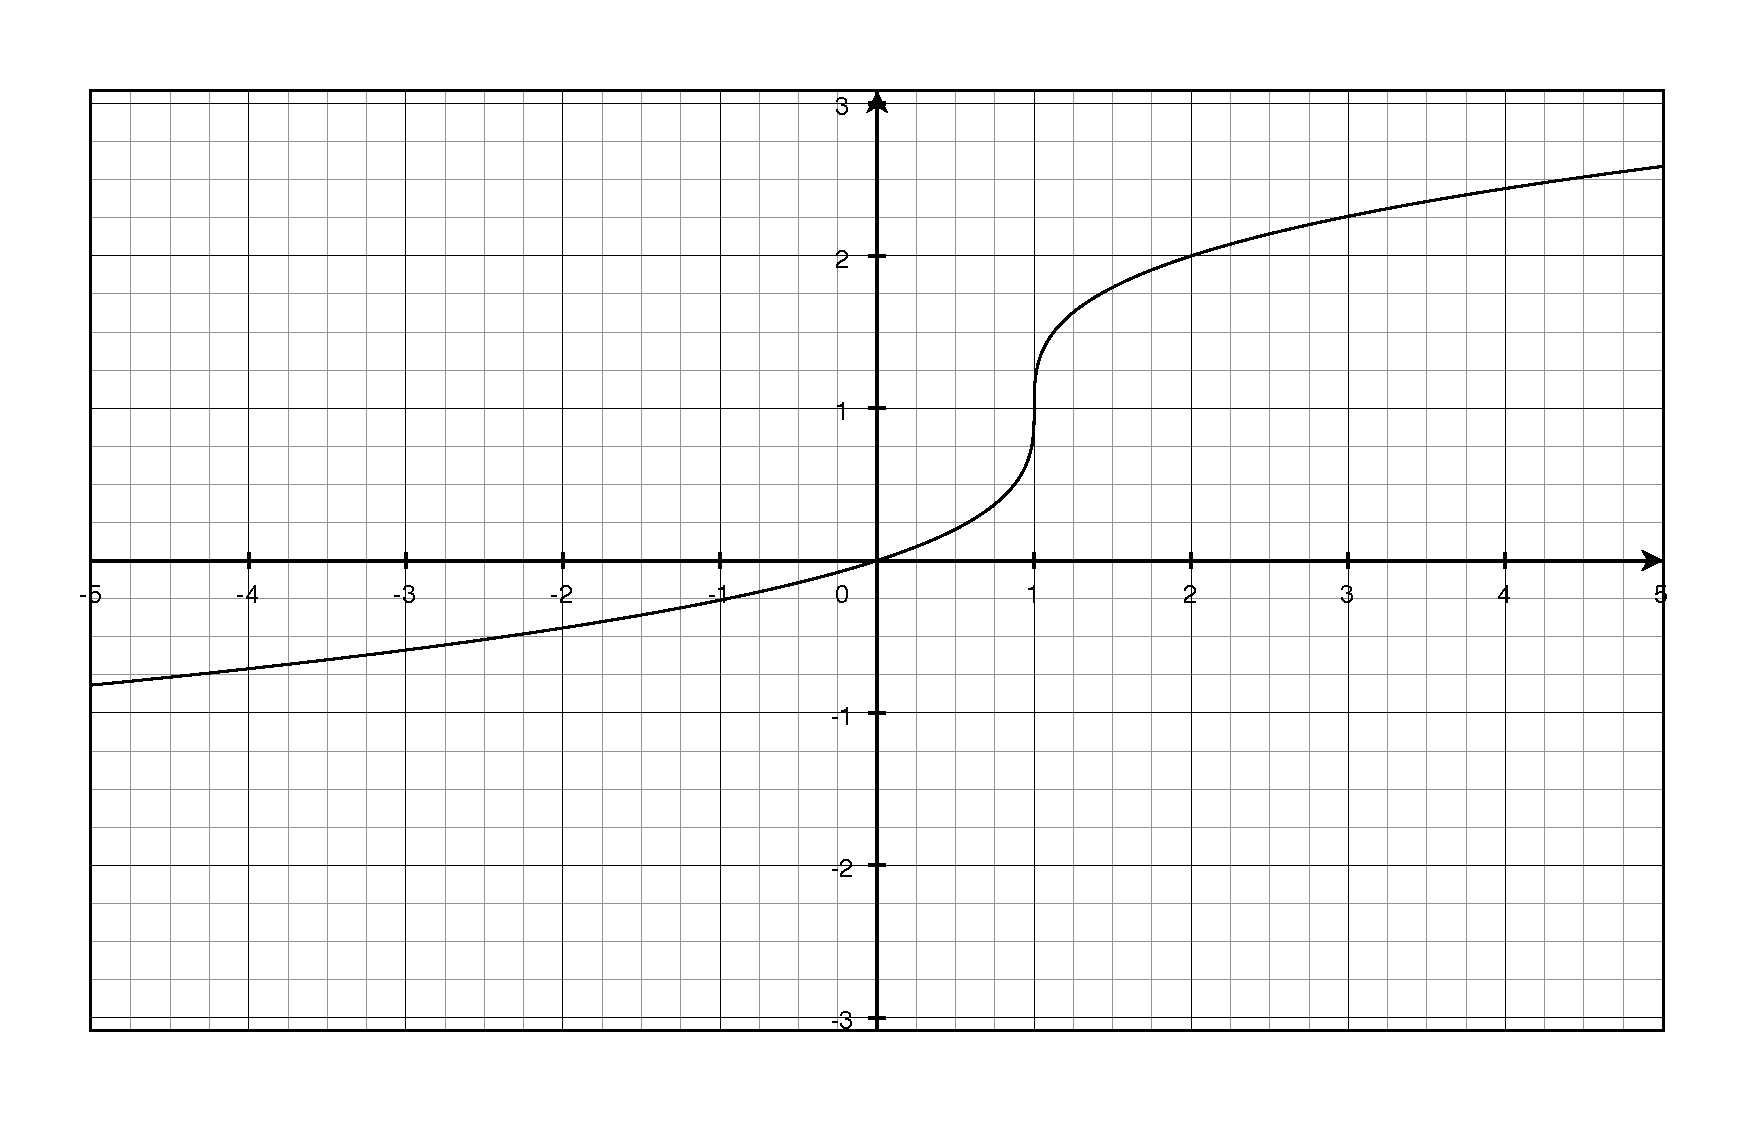
\includegraphics[scale=.3]{question7.eps}
%   \caption*{question 7}
% \end{figure}

% \begin{tabular}{cc}
%   \toprule
%   period & amplitude \\
%   \midrule
%     $\pi$ & $2$ \\
%   \bottomrule
% \end{tabular}

% \printanswers
\excludecomment{comment}

\ifprintanswers 
  \usepackage{2in1, lscape} 
\fi

\author{}
\date{\today}
\title{Math 142 \\ Homework One}

\begin{document}

  \maketitle

  \section{Homework}
  Section 5.1: 7-10, 15-50

  \section{Extra Credit}

  Imagine that you have three boxes. One contains two black marbles, one contains two white marbles, and the third,
  one black marble and one white marble. The boxes were labeled for their contents---BB, BW, WW---but someone switched the
  labels so that every box is now incorrectly labeled. You are allowed to take one marble at a time out of any box,
  without looking inside, and by this process of sampling you are to determine the contents of all three boxes. What is
  the smallest number of drawings needed to do this?
   
  \begin{solution}
    You can identify all the boxes by taking a single marble from the BW box.  You know all the boxes are labeled
    incorrectly, so this box is actually either the WW box or the BB box.  You can tell which of these it is by the color
    of the marble.

    Suppose you draw a white marble.  You now know that the box labeled BW is actually the WW box.  You have two boxes
    left to identify, and you know that they are both labeled incorrectly.  Therefore, the box labeled WW must be the BB
    box and the box labeled BB must be the BW box.
    
    Similar reasoning applies if the marble you draw originally is black.
  \end{solution}

  \ifprintanswers
    \section{Section 5.1}
    \begin{description}

      \item[7]
        \begin{align*}
          \left( \frac{3}{5} \right)^2 + y^2 & = 1 \\
          y                                  & = \pm \frac{4}{5} \\
        \end{align*}

        The point in quadrant III is: $\boxed{ \left( -\frac{3}{5}, -\frac{4}{5} \right) }$.

      \item[8]
        \begin{align*}
          x^2 + \left( - \frac{7}{25} \right)^2 & = 1 \\
          x                                     & = \pm \frac{3 \sqrt{2}}{5} \\
        \end{align*}

        The point in quadrant IV is: $\boxed{ \left( \frac{3 \sqrt{2}}{5}, -\frac{7}{25} \right) }$.

      \item[9]
        \begin{align*}
          x^2 + \left( \frac{1}{3} \right)^2 & = 1 \\
          x                                  & = \pm \frac{2 \sqrt{2}}{3} \\
        \end{align*}

        The point in quadrant IV is: $\boxed{ \left( - \frac{2 \sqrt{2}}{3}, \frac{1}{3} \right) }$.

      \item[10]
        \begin{align*}
          \left( \frac{2}{5} \right)^2 + y^2 & = 1 \\
          y                                  & = \pm \frac{\sqrt{21}}{5} \\
        \end{align*}

        The point in quadrant IV is: $\boxed{ \left( \frac{2}{5}, \frac{\sqrt{21}}{5} \right) }$.

      \item[15]
        \begin{align*}
          x^2 + \left( \frac{2}{3} \right)^2 & = 1 \\
          x                                  & = \pm \frac{\sqrt{5}}{3} \\
        \end{align*}

        The point is: $\boxed{ \left( - \frac{\sqrt{5}}{3}, \frac{2}{3} \right) }$.

      \item[16]
        \begin{align*}
          x^2 + \left( - \frac{\sqrt{5}}{5} \right)^2 & = 1 \\
          x                                  & = \pm \frac{2 \sqrt{5}}{5} \\
        \end{align*}

        The point is: $\boxed{ \left( \frac{2 \sqrt{5}}{5}, \frac{\sqrt{5}}{5} \right) }$.

      \item[17]
        \begin{align*}
          \left( - \frac{\sqrt{2}}{3} \right)^2 + y^2 & = 1 \\
          y                                           & = \pm \frac{\sqrt{7}}{3} \\
        \end{align*}

        The point is: $\boxed{ \left( \frac{\sqrt{2}}{3}, - \frac{\sqrt{7}}{3} \right) }$.

      \item[18]
        \begin{align*}
          \left( - \frac{2}{5} \right)^2 + y^2 & = 1 \\
          y                                    & = \pm \frac{\sqrt{21}}{3} \\
        \end{align*}

        The point is: $\boxed{ \left( - \frac{2}{5}, \frac{\sqrt{21}}{3} \right) }$.

      \item[19]
        \begin{tabular}{cc}
          \toprule
          $t$ & terminal point \\
          \midrule
          $0$ & (1, 0) \\
          $\frac{\pi}{4}$ & $\left( \frac{\sqrt{2}}{2}, \frac{\sqrt{2}}{2} \right)$ \\

          $\frac{\pi}{2}$ & $\left( 0, 1 \right)$ \\
          $\frac{3 \pi}{4}$ & $\left( -\frac{\sqrt{2}}{2}, \frac{\sqrt{2}}{2} \right)$ \\

          $\pi$ & $\left( -1, 0 \right)$ \\
          $\frac{5 \pi}{4}$ & $\left( -\frac{\sqrt{2}}{2}, -\frac{\sqrt{2}}{2} \right)$ \\

          $\frac{3 \pi}{2}$ & $\left( 0, -1 \right)$ \\
          $\frac{7 \pi}{4}$ & $\left( \frac{\sqrt{2}}{2}, -\frac{\sqrt{2}}{2} \right)$ \\
          \bottomrule
        \end{tabular}

      \item[20]
        \begin{tabular}{cc}
          \toprule
          $t$ & terminal point \\
          \midrule
          $0$             & $(1, 0)$ \\
          $\frac{\pi}{6}$ & $\left( \frac{\sqrt{3}}{2}, \frac{1}{2} \right)$ \\
          $\frac{\pi}{3}$ & $\left( \frac{1}{2}, \frac{\sqrt{3}}{2} \right)$ \\

          \midrule
          $\frac{\pi}{2}$   & $(0, 1)$ \\
          $\frac{2 \pi}{3}$ & $\left( -\frac{1}{2}, \frac{\sqrt{3}}{2} \right)$ \\
          $\frac{5 \pi}{6}$ & $\left( -\frac{\sqrt{3}}{2}, \frac{1}{2} \right)$ \\

          \midrule
          $\pi$             & $(-1, 0)$ \\
          $\frac{7 \pi}{6}$ & $\left( -\frac{\sqrt{3}}{2}, -\frac{1}{2} \right)$ \\
          $\frac{4 \pi}{3}$ & $\left( -\frac{1}{2}, -\frac{\sqrt{3}}{2} \right)$ \\

          \midrule
          $\pi$              & $(0, -1)$ \\
          $\frac{5 \pi}{3}$  & $\left( \frac{1}{2}, -\frac{\sqrt{3}}{2} \right)$ \\
          $\frac{11 \pi}{6}$ & $\left( \frac{\sqrt{3}}{2}, -\frac{1}{2} \right)$ \\
          
          \bottomrule
        \end{tabular}

      \item[21] $t = \frac{\pi}{2}$; terminal point: $\boxed{ \left( 0, 1 \right) }$

      \item[22] $t = \frac{3 \pi}{2}$; terminal point: $\boxed{ \left( 0, -1 \right) }$

      \item[23] $t = \frac{5 \pi}{6}$; terminal point: $\boxed{ \left( - \frac{\sqrt{3}}{2}, \frac{1}{2} \right) }$

      \item[24] $t = \frac{7 \pi}{6}$; terminal point: $\boxed{ \left( - \frac{\sqrt{3}}{2}, - \frac{1}{2} \right) }$

      \item[25] $t = -\frac{\pi}{3}$; terminal point: $\boxed{ \left( \frac{1}{2}, - \frac{\sqrt{3}}{2}  \right) }$

      \item[26] $t = \frac{5 \pi}{3}$; terminal point: $\boxed{ \left( \frac{1}{2}, - \frac{\sqrt{3}}{2}  \right) }$

      \item[27] $t = \frac{2 \pi}{3}$; terminal point: $\boxed{ \left( - \frac{1}{2}, \frac{\sqrt{3}}{2}  \right) }$

      \item[28] $t = -\frac{\pi}{2}$; terminal point: $\boxed{ \left( 0, -1 \right) }$

      \item[29] $t = - \frac{3 \pi}{4}$; terminal point: $\boxed{ \left( - \frac{\sqrt{2}}{2}, - \frac{\sqrt{2}}{2}  \right) }$
        
      \item[30] $t = \frac{11 \pi}{6}$; terminal point: $\boxed{ \left( \frac{\sqrt{3}}{2}, - \frac{1}{2}  \right) }$

      \item[31]
        \begin{enumerate}[a]
          \item $\left( - \frac{3}{5}, \frac{4}{5} \right)$
          \item $\left( \frac{3}{5}, - \frac{4}{5} \right)$
          \item $\left( - \frac{3}{5}, - \frac{4}{5} \right)$
          \item $\left( - \frac{3}{5}, - \frac{4}{5} \right)$
        \end{enumerate}

      \item[32]
        \begin{enumerate}[a]
          \item $\left( \frac{3}{4}, - \frac{\sqrt{7}}{4} \right)$
          \item $\left( \frac{3}{4}, \frac{\sqrt{7}}{4} \right)$
          \item $\left( - \frac{3}{4}, \frac{\sqrt{7}}{4} \right)$
          \item $\left( - \frac{3}{4}, - \frac{\sqrt{7}}{4} \right)$
        \end{enumerate}

      \item[33] 
        \begin{enumerate}[a]
          \item $\frac{5 \pi}{4} - \pi   = \boxed{ \frac{\pi}{4} }$
          \item $\frac{7 \pi}{3} - 2 \pi = \boxed{ \frac{\pi}{3} }$
          \item $\frac{4 \pi}{3} - \pi   = \boxed{ \frac{\pi}{3} }$
          \item $\frac{\pi}{6} - 0       = \boxed{ \frac{\pi}{6} }$
        \end{enumerate}
        
      \item[34] 
        \begin{enumerate}[a]
          \item $ \pi - \frac{5 \pi}{6}   = \boxed{ \frac{\pi}{6} }$
          \item $\frac{7 \pi}{6} - \pi    = \boxed{ \frac{\pi}{6} }$
          \item $4 \pi - \frac{11 \pi}{3} = \boxed{ \frac{\pi}{3} }$
          \item $2 \pi - \frac{7 \pi}{4}  = \boxed{ \frac{\pi}{4} }$
        \end{enumerate}
        
      \item[35] 
        \begin{enumerate}[a]
          \item $\pi - \frac{5 \pi}{7} = \boxed{ \frac{2 \pi}{7} }$
          \item $\pi - \frac{7 \pi}{9} = \boxed{ \frac{2 \pi}{9} }$
          \item $\pi - 3         \approx \boxed{ 0.1416 }$
          \item $2 \pi - 5       \approx \boxed{ 1.2832 }$
        \end{enumerate}

      \item[36] 
        \begin{enumerate}[a]
          \item $\frac{11 \pi}{5} - 2 \pi = \boxed{ \frac{\pi}{11} }$
          \item $\frac{9 \pi}{7} - \pi    = \boxed{ \frac{2 \pi}{7} }$
          \item $7 - 2 \pi          \approx \boxed{ 0.7168 }$
          \item $2 \pi - 6          \approx \boxed{ 0.2832 }$
        \end{enumerate}

      \item[37]
        \begin{tabular}[H]{ll}
          \toprule
          reference number & $t = \frac{\pi}{3}$ \\
          \midrule
          terminal point   & $\left( - \frac{1}{2}, \frac{\sqrt{3}}{2} \right)$ \\
          \bottomrule
        \end{tabular}

      \item[38]
        \begin{tabular}[H]{ll}
          \toprule
          reference number & $t = \frac{\pi}{3}$ \\
          \midrule
          terminal point   & $\left( - \frac{1}{2}, - \frac{\sqrt{3}}{2} \right)$ \\
          \bottomrule
        \end{tabular}

      \item[39]
        \begin{tabular}[H]{ll}
          \toprule
          reference number & $t = \frac{\pi}{4}$ \\
          \midrule
          terminal point   & $\left( - \frac{\sqrt{2}}{2}, \frac{\sqrt{2}}{2} \right)$ \\
          \bottomrule
        \end{tabular}

      \item[40]
        \begin{tabular}[H]{ll}
          \toprule
          reference number & $t = \frac{\pi}{3}$ \\
          \midrule
          terminal point   & $\left( \frac{1}{2}, \frac{\sqrt{3}}{2} \right)$ \\
          \bottomrule
        \end{tabular}

      \item[41]
        \begin{tabular}[H]{ll}
          \toprule
          reference number & $t = \frac{\pi}{3}$ \\
          \midrule
          terminal point   & $\left( - \frac{1}{2}, - \frac{\sqrt{3}}{2} \right)$ \\
          \bottomrule
        \end{tabular}

      \item[42]
        \begin{tabular}[H]{ll}
          \toprule
          reference number & $t = \frac{\pi}{6}$ \\
          \midrule
          terminal point   & $\left( - \frac{\sqrt{3}}{2}, \frac{1}{2} \right)$ \\
          \bottomrule
        \end{tabular}

      \item[43]
        \begin{tabular}[H]{ll}
          \toprule
          reference number & $t = \frac{\pi}{4}$ \\
          \midrule
          terminal point   & $\left( - \frac{\sqrt{2}}{2}, - \frac{\sqrt{2}}{2} \right)$ \\
          \bottomrule
        \end{tabular}

      \item[44]
        \begin{tabular}[H]{ll}
          \toprule
          reference number & $t = \frac{\pi}{6}$ \\
          \midrule
          terminal point   & $\left( \frac{\sqrt{3}}{2}, \frac{1}{2} \right)$ \\
          \bottomrule
        \end{tabular}

      \item[45]
        \begin{tabular}[H]{ll}
          \toprule
          reference number & $t = \frac{\pi}{6}$ \\
          \midrule
          terminal point   & $\left( - \frac{\sqrt{3}}{2}, \frac{1}{2} \right)$ \\
          \bottomrule
        \end{tabular}

      \item[46]
        \begin{tabular}[H]{ll}
          \toprule
          reference number & $t = \frac{\pi}{6}$ \\
          \midrule
          terminal point   & $\left( \frac{\sqrt{2}}{2}, \frac{\sqrt{2}}{2} \right)$ \\
          \bottomrule
        \end{tabular}

      \item[47]
        \begin{tabular}[H]{ll}
          \toprule
          reference number & $t = \frac{\pi}{3}$ \\
          \midrule
          terminal point   & $\left( \frac{1}{2}, \frac{\sqrt{3}}{2} \right)$ \\
          \bottomrule
        \end{tabular}

      \item[48]
        \begin{tabular}[H]{ll}
          \toprule
          reference number & $t = \frac{\pi}{6}$ \\
          \midrule
          terminal point   & $\left( - \frac{\sqrt{3}}{2}, - \frac{1}{2} \right)$ \\
          \bottomrule
        \end{tabular}

      \item[49]
        \begin{tabular}[H]{ll}
          \toprule
          reference number & $t = \frac{\pi}{3}$ \\
          \midrule
          terminal point   & $\left( - \frac{1}{2}, - \frac{\sqrt{3}}{2},  \right)$ \\
          \bottomrule
        \end{tabular}

      \item[50]
        \begin{tabular}[H]{ll}
          \toprule
          reference number & $t = \frac{\pi}{3}$ \\
          \midrule
          terminal point   & $\left( \frac{\sqrt{2}}{2}, - \frac{\sqrt{2}}{2} \right)$ \\
          \bottomrule
        \end{tabular}

    \end{description}
  \else
    \vspace{9 cm}
    \begin{quote}
      \begin{em}
        In the beginner's mind there are many possibilities, in the expert's there are few. 
      \end{em}
    \end{quote}
    \hspace{1 cm} --Shunryu Suzuki
  \fi

\end{document}

